\newpage
\appendix
\section*{Appendix}
%conv
\begin{figure}[ht]
\begin{subfigure}{.33\textwidth}
  \centering
  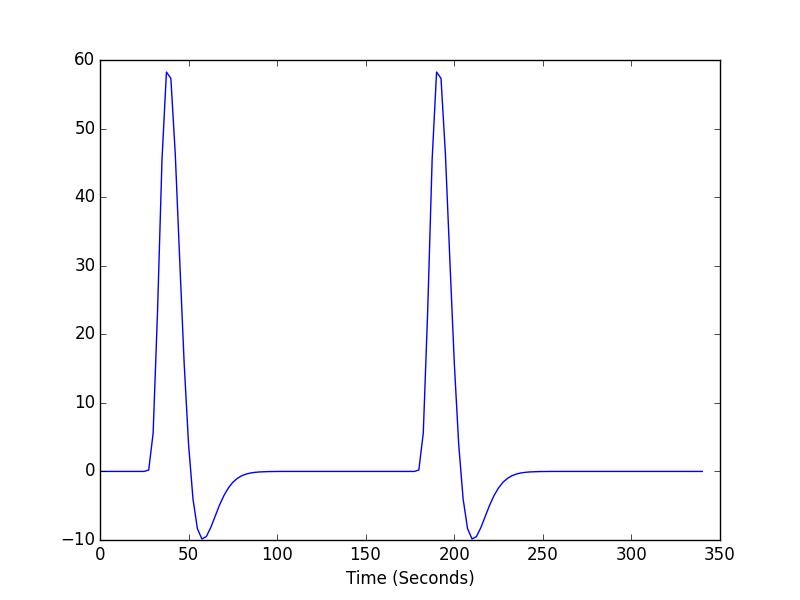
\includegraphics[scale=0.29]{High_resolution_task001_run001_conv001}
\end{subfigure}%
\begin{subfigure}{.33\textwidth}
  \centering
  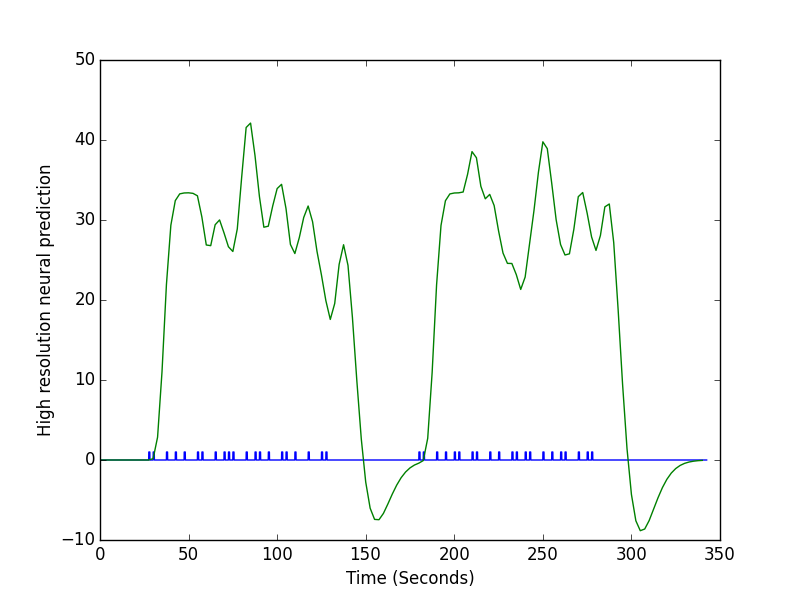
\includegraphics[scale=0.29]{High_resolution_task001_run001_conv002}
\end{subfigure}%
\begin{subfigure}{.33\textwidth}
  \centering
  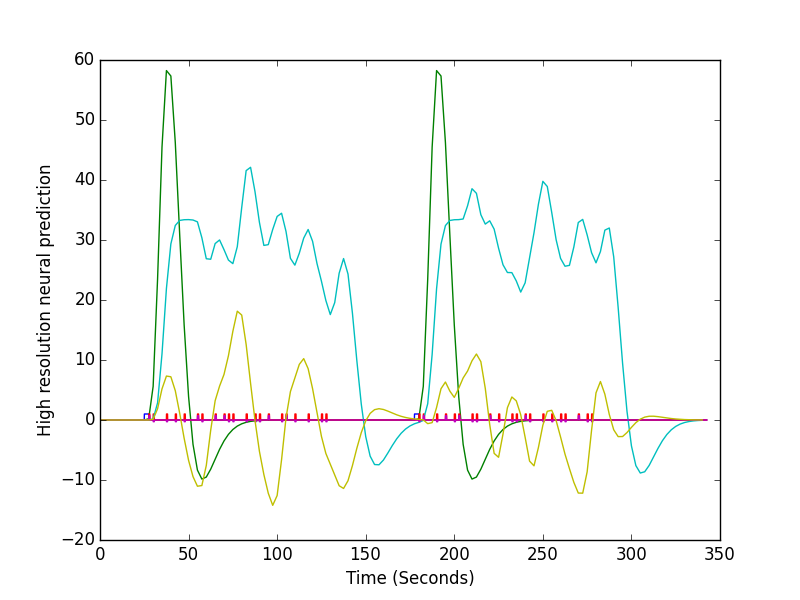
\includegraphics[scale=0.29]{High_resolution_task001_run001_conv003}
\end{subfigure}
\begin{subfigure}{.33\textwidth}
  \centering
  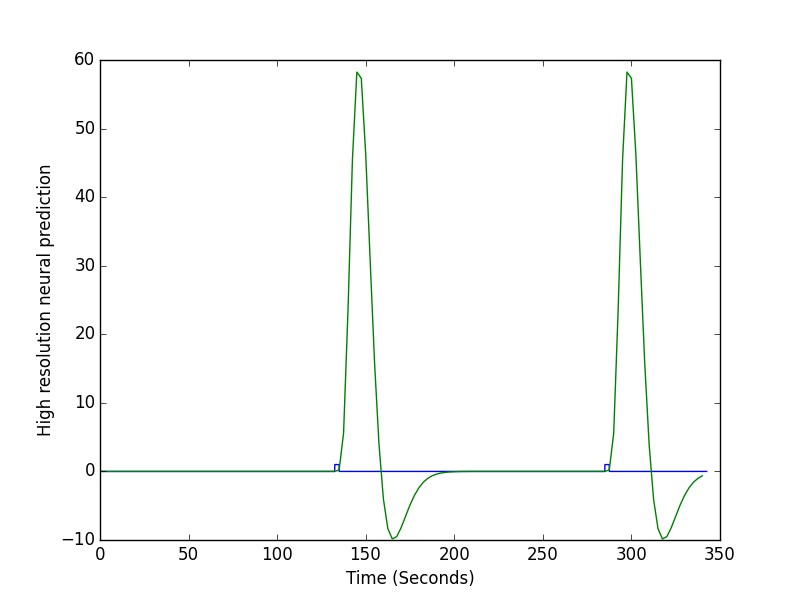
\includegraphics[scale=0.29]{High_resolution_task001_run001_conv004}
\end{subfigure}%
\begin{subfigure}{.33\textwidth}
  \centering
  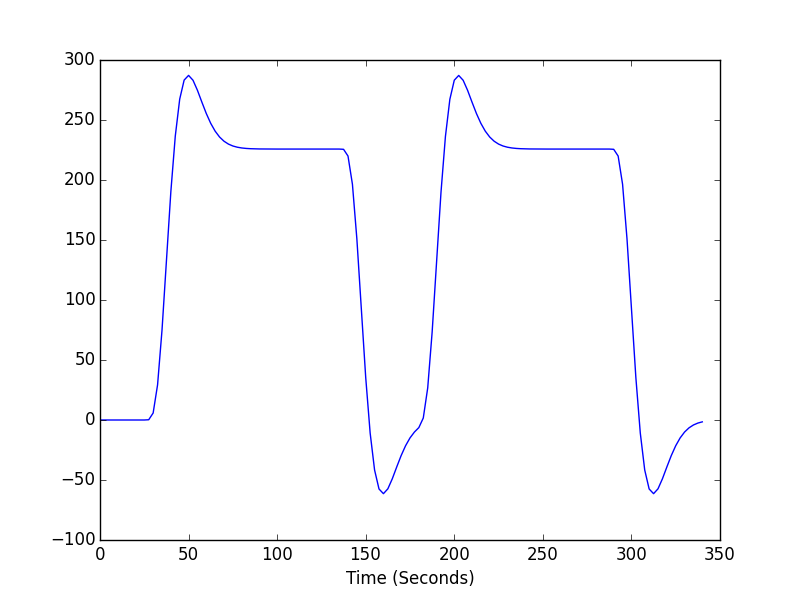
\includegraphics[scale=0.29]{High_resolution_task001_run001_conv005}
\end{subfigure}%
\begin{subfigure}{.33\textwidth}
  \centering
  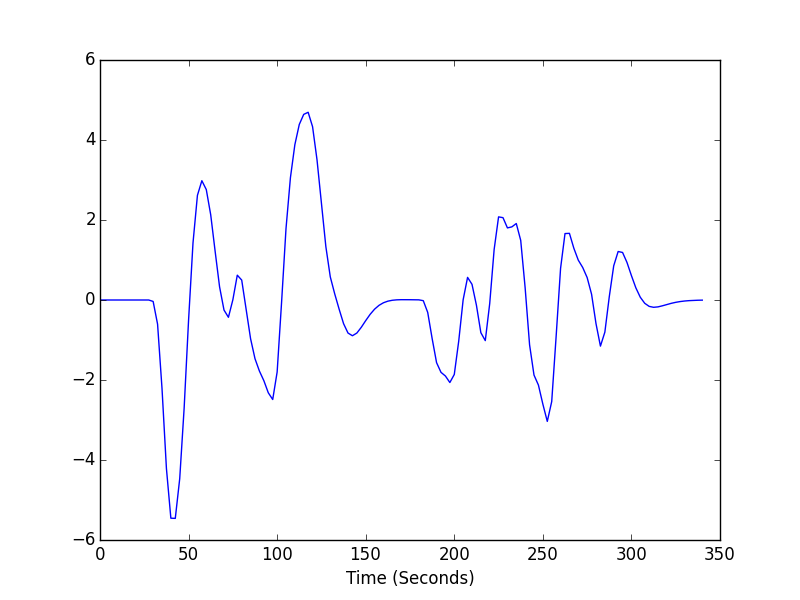
\includegraphics[scale=0.29]{High_resolution_task001_run001_conv006}
\end{subfigure}
\caption{Convolution Response from 6 Conditions\label{fig:ConvRes}}
\end{figure}

\newpage
%block
\begin{figure}[ht]
\centering
\begin{subfigure}{.45\textwidth}
  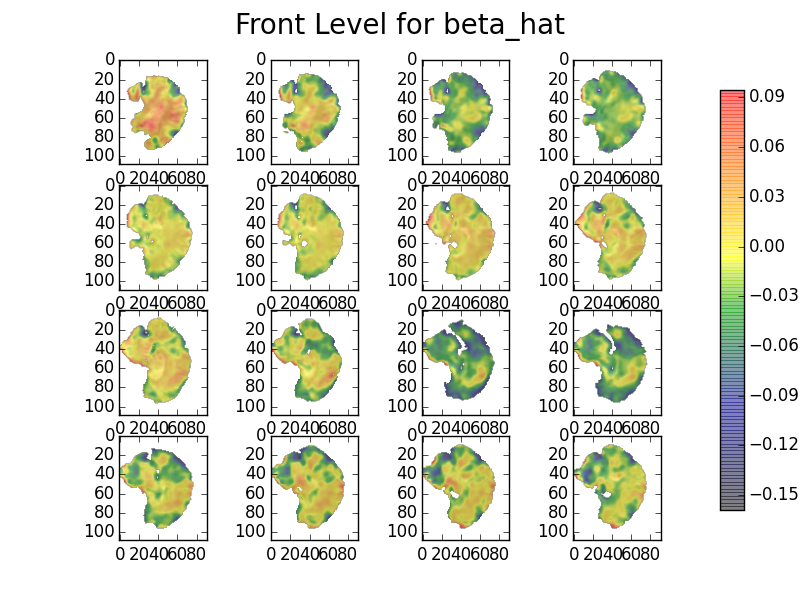
\includegraphics[scale=0.4]{block_beta_front_map}
\end{subfigure}%
\begin{subfigure}{.5\textwidth}
  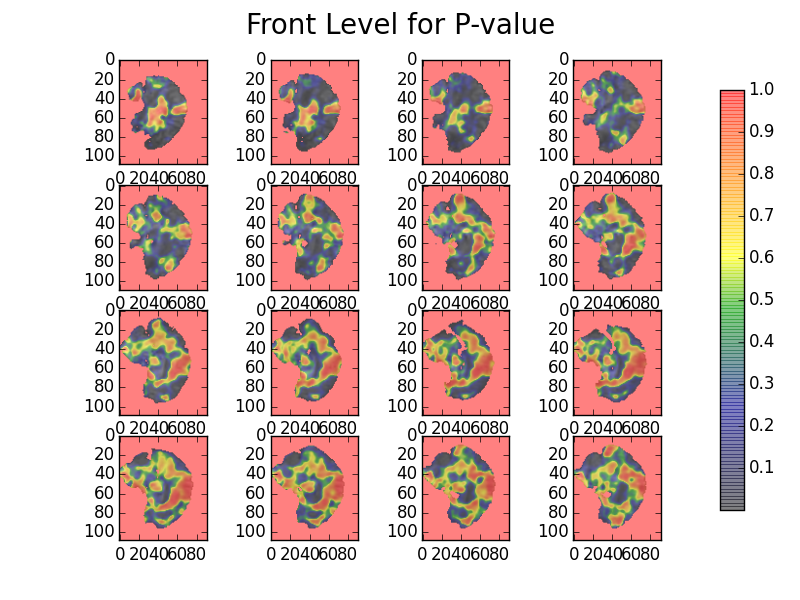
\includegraphics[scale=0.4]{block_p_front_map}
  \centering
\end{subfigure}
\caption{Front Perspective of Brain in Block Design\label{fig:fpBrain}}
\end{figure}

%block
\begin{figure}[ht]
\centering
\begin{subfigure}{.45\textwidth}
  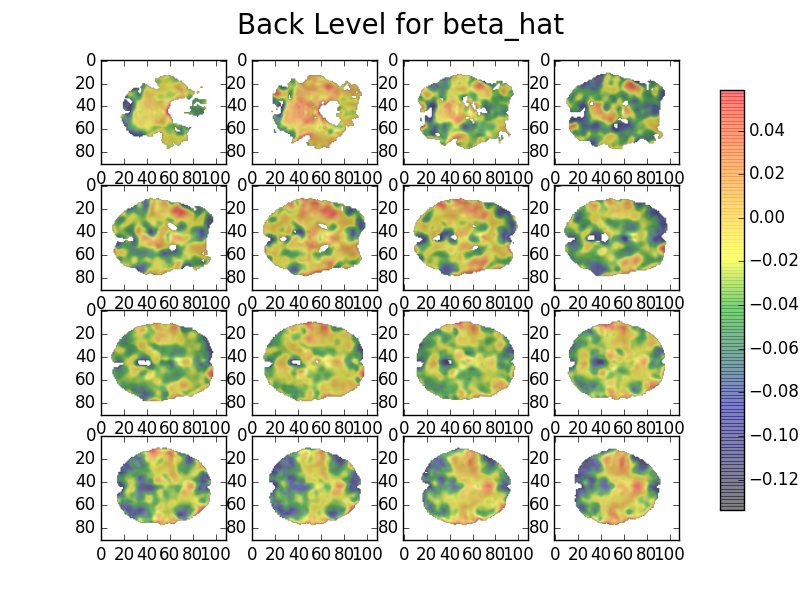
\includegraphics[scale=0.4]{block_beta_back_map}
\end{subfigure}%
\begin{subfigure}{.5\textwidth}
  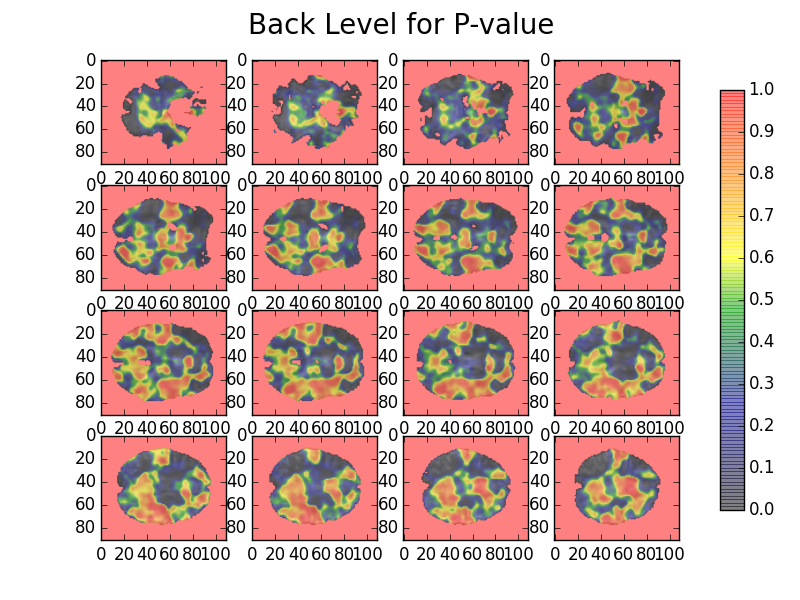
\includegraphics[scale=0.4]{block_p_back_map}
  \centering
\end{subfigure}
\caption{Back Perspective of Brain in Block Design\label{fig:bpBrain}}
\end{figure}




